\chapter{Sel Punca, Regenerasi, dan Penuaan}\label{ch:b3:stem-cells}

Potonglah kaki seekor aksolotl dan dalam dua bulan ia telah menumbuhkan kaki baru,
dengan tulang, otot, saraf, dan kulitnya pada tempat yang benar, lalu ia akan melakukannya
lagi sesering Anda memotongnya. Potonglah seekor cacing pipih planaria menjadi dua puluh keping
dan tiap kepingnya menjadi seekor cacing utuh dalam dua minggu, dengan keping yang tadinya
ekor menumbuhkan sebuah kepala bermata dan berotak. Potonglah sebuah jari manusia
di atas sendi terakhirnya dan ia sembuh sebagai sebuah parut. Namun tubuh manusia
bukanlah tanpa pembaruan: tiap detik ia membuat dua juta sel darah
merah, lapisan ususnya digantikan tiap lima hari, kulitnya
tiap bulan, dan semuanya berasal dari populasi kecil sel
yang membelah sepanjang hidup tanpa menghabiskan dirinya. Bab
ini tentang sel itu --- apa yang menjadikan sebuah \omterm{def:b3:stem-cells:stem}{sel punca}, bagaimana \omterm{def:b3:stem-cells:stem}{ceruknya}
menjaganya, bagaimana seluruh hierarki darah atau ususnya dibangun darinya ---
tentang hewan yang dapat menumbuhkan kembali apa yang tidak dapat kita tumbuhkan dan mengapa, tentang
penemuan bahwa sel mana pun dapat didorong kembali ke keadaan embrionya oleh
empat gen, serta tentang apa yang dikatakan aritmetika pembelahan sel
tentang mengapa kita menua.

\section{Apa itu sel punca}

\begin{definition}[Sel punca dan hierarkinya]\label{def:b3:stem-cells:stem}
\index{sel punca}\index{pembaruan diri}\index{pembelahan tak setangkup}%
\index{pendahulu}\index{sel transit-pelipat ganda}\index{ceruk}
Sebuah \emph{sel punca} punya dua sifat penakrif: ia dapat \emph{membarui diri},
yakni menghasilkan anakan yang berupa sel punca, dan ia dapat menghasilkan anakan
yang berdiferensiasi. Ia dapat melakukan keduanya sekaligus, lewat \emph{pembelahan
tak setangkup}, yakni satu anakan dari tiap jenisnya, dengan nasibnya diputuskan pewarisan
penentu yang tidak sama atau oleh anakan mana yang tetap bersentuhan dengan
\emph{ceruknya} --- yakni lingkungan mikro sel tetangga,
matriks, dan isyarat yang menjaga sebuah sel tetap sel punca; atau ia dapat membelah
secara setangkup, dengan sebagian pembelahannya memberi dua sel punca dan sebagian lain dua sel
yang berdiferensiasi, dengan populasinya ditahan tetap secara rata-rata.
Anakan yang berdiferensiasi biasanya melewati tahap \emph{pendahulu}
atau \emph{transit-pelipat ganda}, yang membelah beberapa kali lagi dengan
potensi yang menyempit sebelum matang: hierarkinya melipatgandakan beberapa
pembelahan sel punca yang lambat menjadi sebuah keluaran yang besar, lalu membatasi cacah
pembelahan yang harus dilakukan tiap sel puncanya. Sel punca dewasa jarang dan lambat
--- sebuah sel punca hematopoietik membelah mungkin sekali setahun, sebuah sel punca
usus sekali sehari --- dan \emph{multipoten}, yakni terbatas pada
garis keturunan jaringannya; \omterm{def:b3:stem-cells:pluripotency}{sel punca embrio}, dari massa sel dalam
blastokistanya, bersifat \emph{pluripoten}, yakni sanggup membuat tiap
jaringan tubuhnya tetapi bukan plasentanya.
\end{definition}

\begin{omfigure}
\begin{tikzpicture}[every node/.style={font=\scriptsize}, >=stealth]
  \node[draw, very thick, rounded corners, fill=omDef!25, align=center] (hsc) at (0,3.6) {sel punca hematopoietik\\$\sim$\num{10000} pada seorang manusia; membelah $\sim$ sekali setahun};
  \node[draw, thick, rounded corners, fill=omDef!12, align=center] (mpp) at (0,2.4) {pendahulu multipoten};
  \node[draw, thick, rounded corners, fill=omThm!15, align=center] (cmp) at (-3.2,1.2) {pendahulu mieloid};
  \node[draw, thick, rounded corners, fill=omProp!20, align=center] (clp) at (3.2,1.2) {pendahulu limfoid};
  \node[align=center, font=\tiny] (e) at (-5.4,-0.4) {eritrosit\\$2\times 10^{11}$/hari};
  \node[align=center, font=\tiny] (pl) at (-3.6,-0.4) {keping darah\\(megakariosit)};
  \node[align=center, font=\tiny] (g) at (-1.8,-0.4) {granulosit\\$10^{11}$/hari};
  \node[align=center, font=\tiny] (m) at (-0.2,-0.4) {monosit,\\makrofag};
  \node[align=center, font=\tiny] (b) at (1.8,-0.4) {sel B};
  \node[align=center, font=\tiny] (t) at (3.4,-0.4) {sel T};
  \node[align=center, font=\tiny] (nk) at (5.0,-0.4) {sel NK};
  \draw[->, thick] (hsc) -- (mpp); \draw[->, thick] (mpp) -- (cmp); \draw[->, thick] (mpp) -- (clp);
  \foreach \x in {e,pl,g,m} { \draw[->, thick] (cmp) -- (\x); }
  \foreach \x in {b,t,nk} { \draw[->, thick] (clp) -- (\x); }
  \draw[->, thick, omDef!70!black] (hsc.west) .. controls (-3.0,4.4) and (-3.0,3.0) .. (hsc.south west) node[pos=0.5, left, font=\tiny, omDef!70!black, align=right] {pembaruan diri};
  \node[right, align=left, font=\tiny] at (4.4,3.6) {tiap tingkatnya membelah lebih sering\\dan potensinya lebih sempit;\\$\sim 20$ pembelahan dari sel punca\\ke sel merah, sehingga satu pembelahan\\sebuah sel punca menghasilkan $\sim 10^{6}$ sel};
\end{tikzpicture}

{\small Hierarki hematopoietiknya. Beberapa ribu \omterm{def:b3:stem-cells:stem}{sel punca} yang lambat di
dalam sumsumnya memberi makan \omterm{def:b3:stem-cells:stem}{pendahulu} yang membelah cepat lalu berkomitmen berangsur,
sehingga keluaran sejuta juta sel tiap hari nyaris tidak berongkos apa pun bagi \omterm{def:b3:stem-cells:stem}{sel
puncanya}.}
\end{omfigure}

\begin{proof}[Bukti eksperimental]
Till dan McCulloch (1961) menyuntikkan sel sumsum ke dalam mencit yang
disinari sampai mematikan lalu mencacah bintil yang muncul pada limpanya
sepuluh hari kemudian: masing-masing adalah sebuah koloni sel darah dari beberapa garis keturunan,
dengan cacahnya sebanding dengan sel yang disuntikkan, dan menandai kromosom sel
donornya menunjukkan tiap koloninya sebuah klona --- sebuah sel
tunggal telah membuat sel merah, granulosit, dan keping darah, dan sebagian koloninya
memuat sel yang dapat menyemai koloni baru pada seekor mencit kedua:
yakni \omterm{def:b3:stem-cells:stem}{pembaruan diri} dan multipotensi di dalam satu sel, yakni definisi operasional
sebuah \omterm{def:b3:stem-cells:stem}{sel punca}, dan dasar pencangkokan sumsum tulang. Barker dan
Clevers (2007) menandai sel yang mengungkapkan gen \emph{Lgr5} pada pangkal
kripta ususnya dengan sebuah warna yang dapat diwariskan lalu menyaksikan, selama berminggu-minggu,
warnanya mendaki kriptanya lalu mengisi jonjot utuh: sel yang ditandainya adalah
\omterm{def:b3:stem-cells:stem}{sel punca} ususnya, dan salah satunya, yang dibiakkan di dalam sebuah gel dengan
ketiga faktor pertumbuhan yang benar, tumbuh menjadi sebuah usus mungil, yakni sebuah
\emph{\omterm{def:b3:stem-cells:pluripotency}{organoid}}, dengan kripta dan jonjotnya sendiri (Sato, 2009).
\end{proof}

\begin{proposition}[Ceruk dan kriptanya]\label{prop:b3:stem-cells:crypt}
\index{kripta}\index{Lgr5}\index{sel Paneth}%
\index{pengisyaratan Wnt}\index{hanyutan netral}
\emph{Kripta} usus adalah \omterm{def:b3:stem-cells:stem}{ceruk} yang paling dipahami. Pada pangkalnya
sekitar empat belas \omterm{def:b3:stem-cells:stem}{sel punca} \emph{Lgr5} duduk terjepit di antara \omterm{prop:b3:stem-cells:crypt}{sel Paneth},
yang menyekresikan isyarat Wnt dan Notch serta faktor pertumbuhan yang menjaganya
tetap \omterm{def:b3:stem-cells:stem}{sel punca}; sebuah \omterm{def:b3:stem-cells:stem}{sel punca} yang terdorong ke atas lepas dari sentuhan \omterm{prop:b3:stem-cells:crypt}{sel
Panethnya} kehilangan isyaratnya dalam beberapa garis tengah sel lalu menjadi sebuah
\omterm{def:b3:stem-cells:stem}{sel transit-pelipat ganda}, yang membelah empat atau lima kali di dalam kriptanya
lalu berdiferensiasi menjadi sel penyerap dan penyekresi yang
berpindah naik ke jonjotnya lalu dilepaskan dari pucuknya lima hari kemudian. \omterm{def:b3:stem-cells:stem}{Sel
puncanya} membelah secara setangkup, sekitar sekali sehari, lalu bersaing memperebutkan
ruang \omterm{def:b3:stem-cells:stem}{ceruknya} yang terbatas: secara kebetulan satu klona berkembang dan yang lain
hilang, sehingga dalam beberapa bulan tiap kriptanya berasal dari
sebuah \omterm{def:b3:stem-cells:stem}{sel punca} tunggal --- yakni \emph{\omterm{prop:b3:stem-cells:crypt}{hanyutan netral}} pada skala sebuah kripta, yakni sebuah
jalan acak dengan batas yang menyerap. \omterm{def:b3:stem-cells:stem}{Ceruknya}, bukan selnya, yang memegang
kepuncaannya: taruhlah sebuah sel yang berdiferensiasi kembali bersentuhan dengan isyarat
Paneth sesudah cedera dan ia dapat berbalik; ambillah \omterm{def:b3:stem-cells:stem}{sel puncanya} keluar lalu
berilah ia isyaratnya di dalam sebuah cawan dan ia membuat sebuah \omterm{def:b3:stem-cells:pluripotency}{organoid}. Sumsum tulang,
folikel rambut, testis, dan zona \omterm{def:b3:stem-cells:stem}{sel punca} saraf otaknya
mengikuti logika yang sama dengan isyarat yang berbeda.
\end{proposition}
\begin{proof}[Bukti eksperimental]
Snippert dan rekannya (2010) menandai \omterm{def:b3:stem-cells:stem}{sel punca} kripta dengan sebuah
``konfeti'' empat warna acak; kriptanya mula-mula berwarna-warni
lalu telah menjadi berwarna tunggal dalam beberapa bulan, pada sebuah laju yang memadani
pembelahan setangkup dan persaingan netral di antara sekitar empat belas sel
--- alih-alih \omterm{def:b3:stem-cells:stem}{pembelahan tak setangkup}, yang akan menjaga tiap warnanya
tanpa batas. Menyingkirkan \omterm{prop:b3:stem-cells:crypt}{sel Panethnya} menyusutkan kumpulan \omterm{def:b3:stem-cells:stem}{sel puncanya};
menyingkirkan isyarat Wntnya mengosongkan kriptanya dalam beberapa hari.
\end{proof}

\begin{omfigure}
\begin{tikzpicture}[every node/.style={font=\scriptsize}, >=stealth]
  % crypt-villus
  \draw[very thick, omDef] (0,-2.6) .. controls (0,-0.4) and (0.4,0) .. (0.8,0) -- (0.8,3.6) .. controls (0.8,4.1) and (1.6,4.1) .. (1.6,3.6) -- (1.6,0) .. controls (2.0,0) and (2.4,-0.4) .. (2.4,-2.6);
  \draw[very thick, omDef] (0,-2.6) arc[start angle=180, end angle=360, radius=1.2];
  % stem cells at base
  \foreach \a in {200,230,260,290,320} { \fill[omThm!60] ({1.2+1.05*cos(\a)},{-2.6+1.05*sin(\a)}) circle (0.14); }
  \foreach \a in {215,245,275,305} { \fill[omMeth!60] ({1.2+0.75*cos(\a)},{-2.6+0.75*sin(\a)}) circle (0.13); }
  \node[right, align=left, font=\tiny] at (2.6,-3.4) {pangkal: $\sim 14$ sel punca \emph{Lgr5} (merah)\\terjepit di antara sel Paneth (hijau),\\yang memasok Wnt, Notch, EGF};
  % TA zone
  \foreach \y in {-1.8,-1.3,-0.8,-0.3} { \fill[omProp!50] (0.35,\y) circle (0.11); \fill[omProp!50] (2.05,\y) circle (0.11); }
  \node[right, align=left, font=\tiny] at (2.6,-1.1) {zona transit-pelipat ganda:\\4--5 pembelahan, sekali sehari,\\di luar isyarat Panethnya};
  % villus cells
  \foreach \y in {0.4,1.0,1.6,2.2,2.8} { \fill[omDef!40] (0.95,\y) circle (0.1); \fill[omDef!40] (1.45,\y) circle (0.1); }
  \node[right, align=left, font=\tiny] at (2.6,1.8) {jonjot: sel yang berdiferensiasi\\berpindah naik lalu dilepaskan\\dari pucuknya sesudah $\sim 5$ hari};
  \node[left, font=\tiny] at (-0.1,-2.6) {kripta}; \node[left, font=\tiny] at (0.7,3.9) {pucuk jonjot};
  % confetti panel
  \begin{scope}[shift={(8.8,0.2)}]
    \node[above, align=center] at (0,1.3) {hanyutan netral di dalam ceruknya};
    \foreach \i/\cols in {0/{omDef!60,omThm!60,omMeth!60,omProp!60,omDef!60,omThm!60}, 1/{omDef!60,omDef!60,omThm!60,omThm!60,omThm!60,omProp!60}, 2/{omThm!60,omThm!60,omThm!60,omThm!60,omDef!60,omThm!60}, 3/{omThm!60,omThm!60,omThm!60,omThm!60,omThm!60,omThm!60}} {
      \foreach [count=\j] \c in \cols { \fill[\c] ({\j*0.36-1.26},{1.0-\i*0.7}) circle (0.15); }
    }
    \node[left, font=\tiny] at (-1.35,1.0) {minggu 0}; \node[left, font=\tiny] at (-1.35,0.3) {minggu 4}; \node[left, font=\tiny] at (-1.35,-0.4) {minggu 12}; \node[left, font=\tiny] at (-1.35,-1.1) {beberapa bulan};
    \node[below, align=center, font=\tiny] at (0,-1.75) {klonanya bersaing memperebutkan sejumlah tempat\\yang tetap; satu menang secara kebetulan};
  \end{scope}
\end{tikzpicture}

{\small Kripta sebagai sebuah \omterm{def:b3:stem-cells:stem}{ceruk}. Kepuncaan adalah sebuah tempat: sel yang bersentuhan dengan
isyarat \omterm{prop:b3:stem-cells:crypt}{sel Panethnya} tetap \omterm{def:b3:stem-cells:stem}{sel punca}, sel yang terdorong lepas dari sentuhannya
memulai perjalanan lima hari ke pucuk jonjotnya. Ditandai dengan warna
acak, \omterm{def:b3:stem-cells:stem}{sel punca} sebuah kripta hanyut menjadi sebuah klona tunggal dalam beberapa bulan.}
\end{omfigure}

\section{Pluripotensi dan pemrograman ulang}

\begin{definition}[Embrio, terimbas, dan terbiak]\label{def:b3:stem-cells:pluripotency}
\index{sel punca embrio}\index{pluripotensi}%
\index{sel punca pluripoten terimbas}\index{pemrograman ulang}\index{organoid}
\emph{\omterm{def:b3:stem-cells:stem}{Sel punca} embrio} (Evans, Kaufman, Martin, 1981, mencit;
Thomson, 1998, manusia) adalah sel massa sel dalam yang dijaga tetap membelah di dalam
biakan tanpa berdiferensiasi, oleh isyarat (LIF, atau FGF dan aktivin)
yang memelihara sebuah inti faktor transkripsi --- Oct4, Sox2, Nanog ---
yang saling mengaktifkan lalu menekan gen tiap garis keturunannya.
Ketika disuntikkan ke dalam sebuah blastokista, mereka bergabung dengan embrionya lalu menyumbang pada semua
jaringannya, termasuk garis nutfahnya, dan begitulah mencit \omterm{def:b3:genetic-engineering:transgenic}{penidakaktifan gen}
dibuat: ubahlah sebuah gen di dalam selnya, lalu buatlah seekor mencit darinya. Pemindahan
inti pada jilid Tahun~2 menunjukkan bahwa sebuah inti yang berdiferensiasi dapat
disetel ulang oleh sitoplasma telurnya; Takahashi dan Yamanaka (2006) menemukan apa yang
melakukan penyetelan ulangnya. Dari dua puluh empat gen calonnya, empat --- \emph{Oct4},
\emph{Sox2}, \emph{Klf4}, \emph{c-Myc} --- yang dimasukkan bersama lewat
\omterm{def:b3:virology:virus}{virus} ke dalam fibroblas kulit, mengubah sekitar satu sel dari seribu
sepanjang tiga minggu menjadi sebuah \emph{\omterm{def:b3:stem-cells:stem}{sel punca} pluripoten terimbas}
yang tak terbedakan dari sel embrio, yang sanggup membentuk tiap jaringan dan
seekor mencit utuh. \emph{Pemrograman ulang} lambat dan tak mangkus sebab
faktornya harus membuka \omterm{def:b3:chromatin-epigenetics:nucleosome}{kromatin} yang ditutup bertahun-tahun diferensiasi, dan
selnya melewati sebuah fase acak yang di dalamnya kebanyakan macet; ia
juga, pada asasnya, sebuah jalan dari sel pasiennya sendiri ke jaringan mana pun.
Tambahkanlah isyarat yang benar dalam urutan yang benar dan sel pluripoten di dalam sebuah
cawan mengulang perkembangannya: otot jantung yang berdenyut, neuron
dopamin untuk dicangkokkan ke dalam sebuah otak Parkinson, sel \omterm{def:b3:sensory-systems:retina}{retina}, dan
\emph{organoid} --- yakni jaringan tiga dimensi yang menata diri selebar beberapa
milimeter, berupa usus, ginjal, hati, dan otak, dengan
arsitektur dan jenis sel organnya, yang di dalamnya perkembangan dan penyakit manusia
dapat disaksikan dan obat diuji.
\end{definition}

\begin{omfigure}
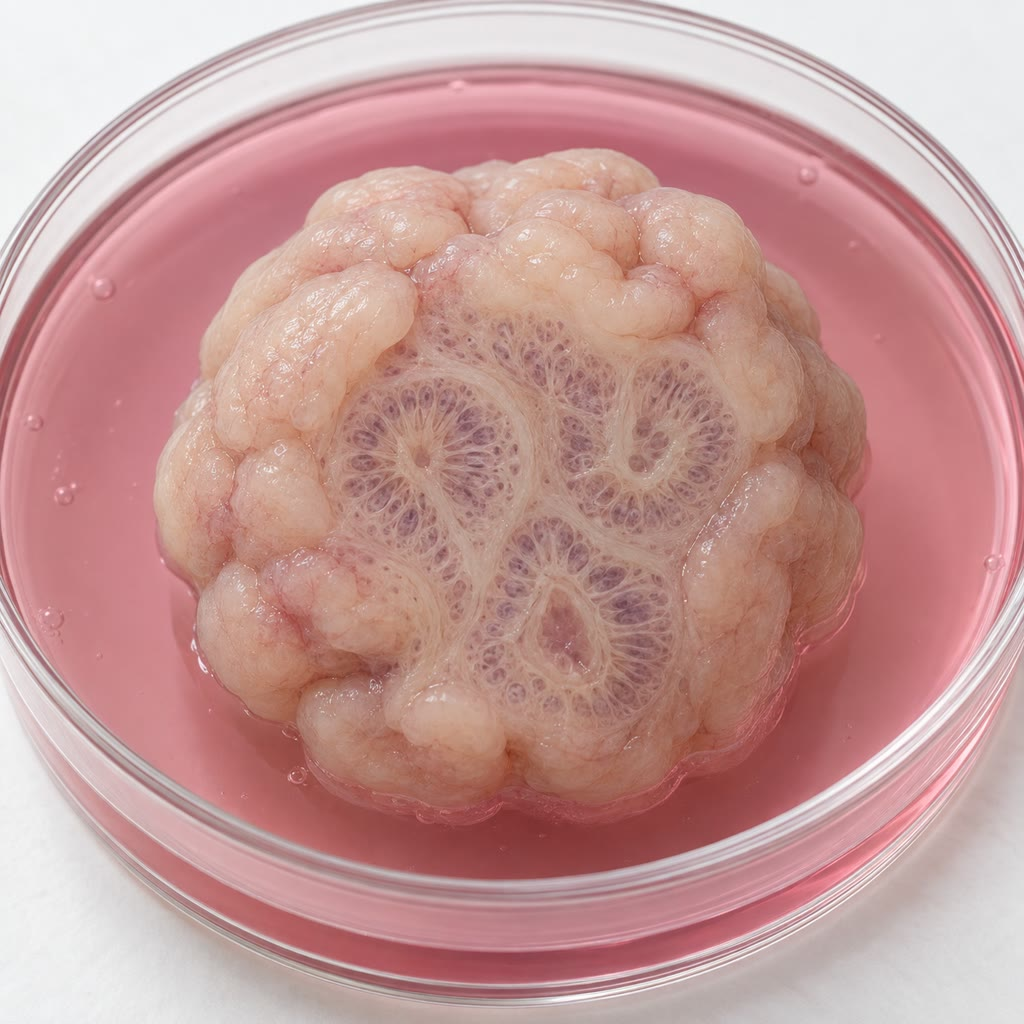
\includegraphics[width=0.4\linewidth]{images/book5/ai/b5-24-brain-organoid.jpg}\hspace{0.04\linewidth}
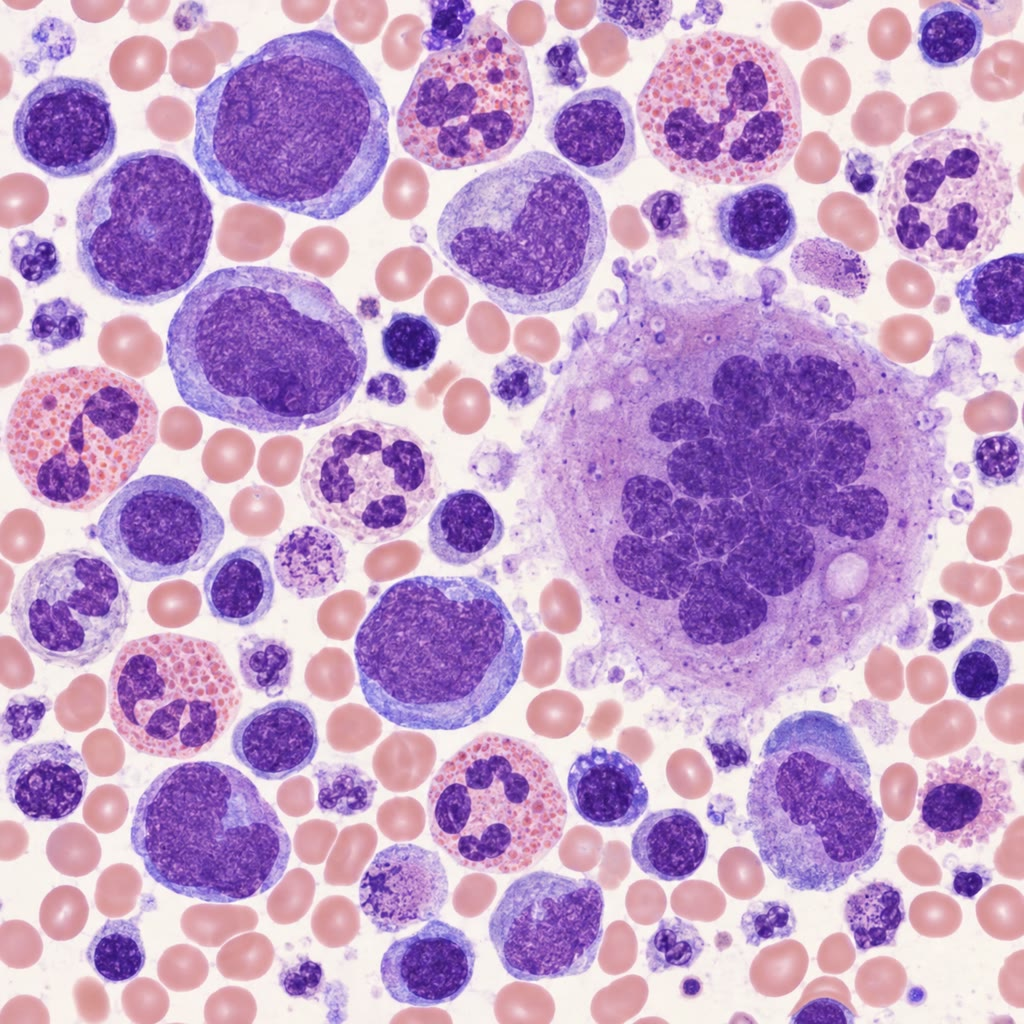
\includegraphics[width=0.4\linewidth]{images/book5/ai/b5-24-bone-marrow-smear.jpg}

{\small Kiri: sebuah \omterm{def:b3:stem-cells:pluripotency}{organoid} otak yang ditumbuhkan dari sel pluripoten manusia
--- yakni beberapa milimeter jaringan serupa korteks yang menata diri, dengan
rongga serupa bilik otak dan neuron yang berlapis. Kanan: sebuah apusan sumsum
tulang, yakni hierarki gambar pertamanya yang terlihat sekaligus: blas,
granulosit yang mematang, \omterm{def:b3:stem-cells:stem}{pendahulu} sel merah, dan sebuah megakariosit.}
\end{omfigure}

\begin{method}[Penelusuran garis keturunan]\label{met:b3:stem-cells:tracing}
\index{penelusuran garis keturunan}\index{rekombinase Cre}
Untuk menemukan sel mana yang menjadi \omterm{def:b3:stem-cells:stem}{sel punca} sebuah jaringan: (1) pilihlah sebuah gen
yang diungkapkan sel calonnya lalu taruhlah di bawah promotornya sebuah
rekombinase terimbas (Cre-ER, yang aktif hanya ketika tamoksifen diberikan);
(2) pada hewan yang sama, sebuah gen pelapor yang menjadi aktif secara tetap
ketika rekombinasenya memotong sebuah kaset penghenti keluar darinya --- yakni sebuah
warna yang diwarisi tiap keturunannya; (3) berilah satu dosis
tamoksifen untuk menandai sel calonnya pada satu saat; (4) panenlah
jaringannya pada selang waktu tertentu lalu nilailah klona yang ditandainya: sebuah klona yang tumbuh,
bertahan berbulan-bulan, dan memuat tiap jenis sel jaringannya berasal
dari sebuah \omterm{def:b3:stem-cells:stem}{sel punca}; sebuah klona yang dilepaskan dalam sepekan berasal dari sebuah
sel transit. (5) Dengan sebuah pelapor berwarna banyak, ikutilah persaingan
antarklonanya. (6) Ujilah fungsinya secara langsung dengan membunuh sel yang ditandainya
memakai sebuah reseptor racun yang diungkapkan di bawah promotor yang sama, lalu lihatlah
apakah jaringannya gagal membarui diri.
\end{method}

\section{Regenerasi}

\begin{definition}[Bagaimana hewan menumbuhkan kembali]\label{def:b3:stem-cells:regeneration}
\index{regenerasi}\index{neoblas}\index{blastema}%
\index{dediferensiasi}\index{pertumbuhan pengimbang}
Regenerasi menempuh tiga jalan. \emph{Hydra} dan planaria bergantung pada
\omterm{def:b3:stem-cells:stem}{sel punca} dewasa yang pluripoten: \emph{neoblas} seekor planaria, yakni seperlima
selnya, adalah satu-satunya sel yang membelah yang dipunyainya, yang berpindah ke sebuah luka,
lalu membangun kembali bagian mana pun yang hilang dengan dipandu isyarat kedudukan (sebuah landaian
Wnt memberi tahu kepingnya ujung mana yang ekornya; halangilah ia dan sebuah keping ekor
menumbuhkan sebuah kepala kedua). Salamander membangun kembali sebuah anggota badan dari sebuah
\emph{blastema}, yakni sebuah tudung sel yang membelah pada tunggulnya yang terbentuk kebanyakan lewat
\emph{dediferensiasi}: serat ototnya terpecah menjadi sel berinti
tunggal, sel tulang rawan dan sel penyambungnya kembali ke sebuah keadaan \omterm{def:b3:stem-cells:stem}{pendahulu},
dengan masing-masing mengingat jaringan asalnya dan kedudukannya sepanjang anggota badannya,
lalu blastemanya menjalankan ulang acara anggota badan embrionya di bawah epidermis
lukanya dan sarafnya, yang kehadirannya dituntut (buanglah sarafnya dari
tunggulnya dan tidak ada yang tumbuh). Ikan zebra menumbuhkan kembali sirip dan jantungnya dengan cara
yang sama, dengan sel otot jantungnya yang selamat membelah untuk menggantikan seperlima
biliknya dalam sebulan. Mamalia sedikit sekali melakukan ini: hatinya menumbuhkan kembali
massanya sesudah dua pertiganya dibuang, tetapi lewat sel yang tersisa
membelah di tempat (\emph{pertumbuhan pengimbang}), bukan lewat membangun kembali
lobus yang hilang; sebuah ujung jari beregenerasi pada anak; ranggah rusanya
tumbuh baru tiap tahun dari sebuah periosteum bersel punca. Mengapa tidak lebih adalah sebuah
pertanyaan tentang pertukaran: tanggapan luka mamalia --- pembekuan yang cepat,
\omterm{def:b3:innate-immunity:inflammation}{peradangan}, parut fibroblas --- menutup sebuah luka dengan cepat terhadap infeksi
dan kehilangan darah, dan parutnya menutup jalan bagi blastemanya; dan sel yang
dapat berdediferensiasi lalu membelah sesuka hati adalah sel yang dapat menjadi
\omterm{def:b3:cancer-biology:hallmarks}{kanker}, yakni sebuah risiko yang mungkin tidak terjangkau seekor hewan berdarah panas yang berumur panjang.
\end{definition}

\begin{omfigure}
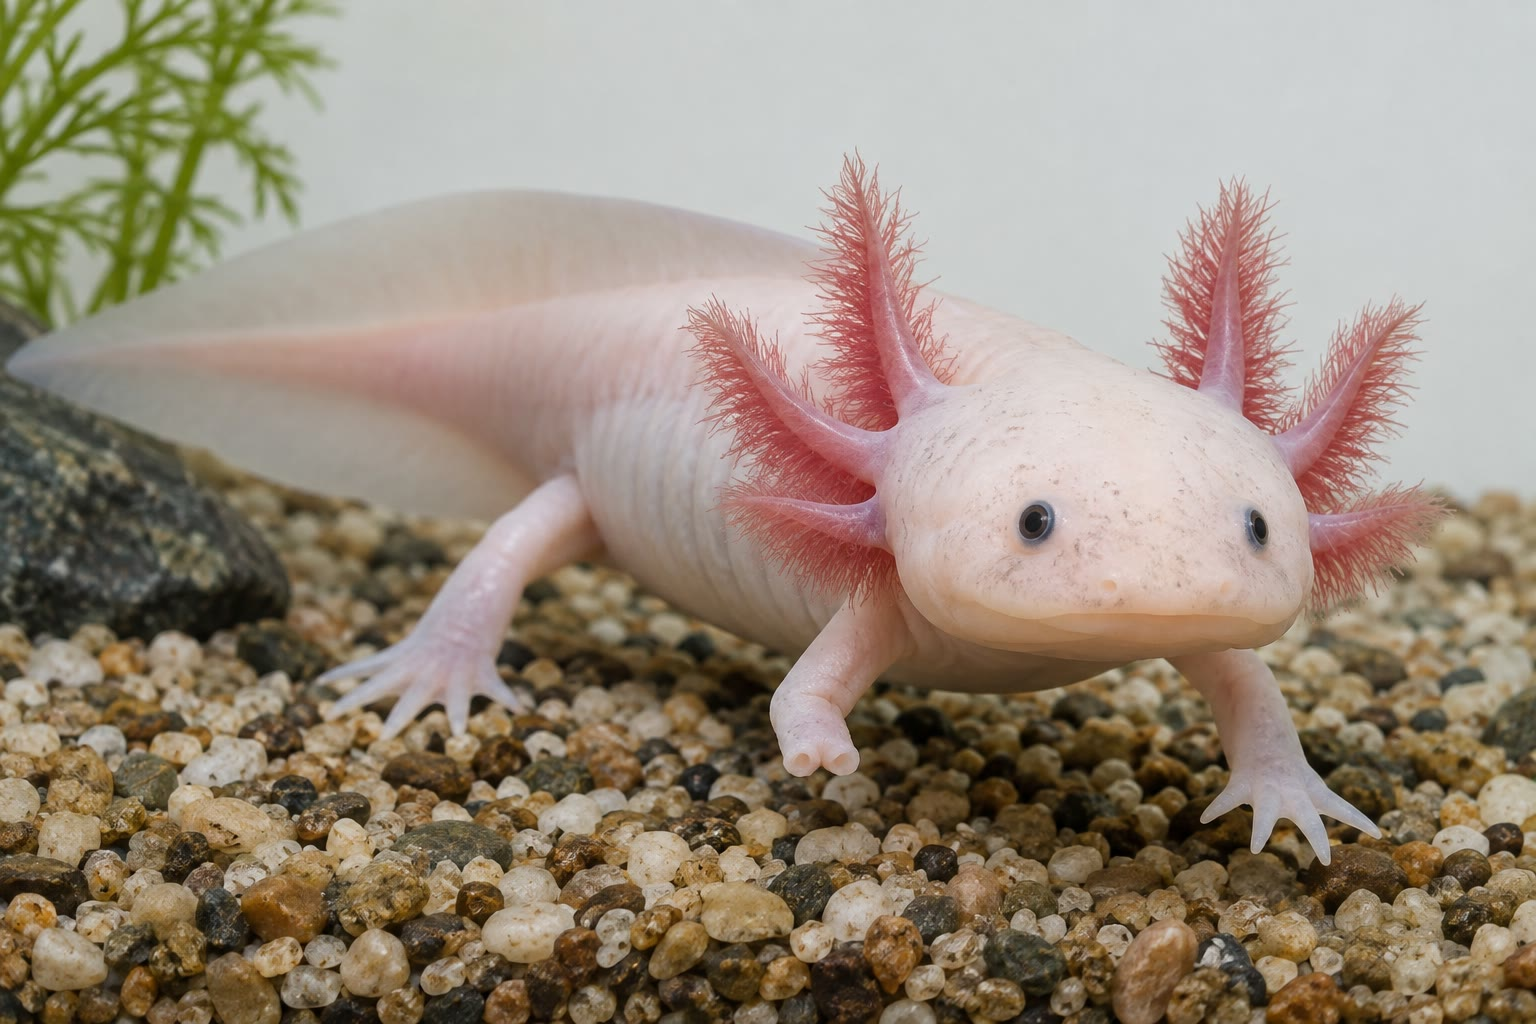
\includegraphics[width=0.46\linewidth]{images/book5/ai/b5-24-axolotl.jpg}\hspace{0.04\linewidth}
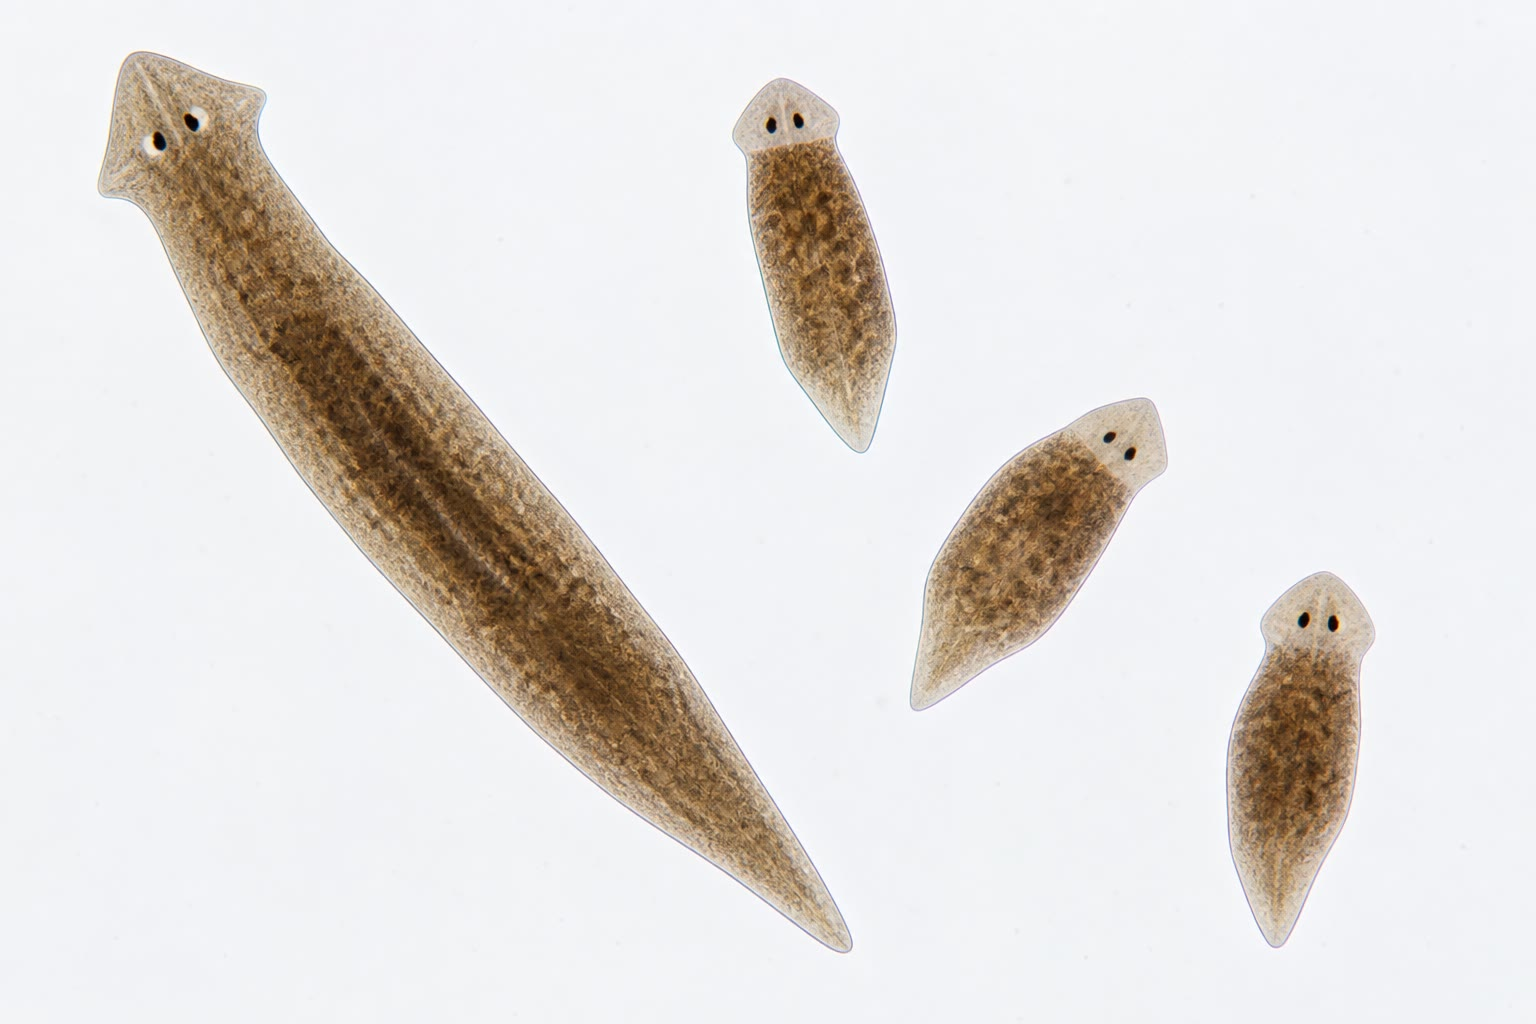
\includegraphics[width=0.46\linewidth]{images/book5/ai/b5-24-planarian-regeneration.jpg}

{\small Kiri: seekor aksolotl, yang menumbuhkan kembali sebuah anggota badan dalam dua bulan dari sebuah
\omterm{def:b3:stem-cells:regeneration}{blastema} sel yang berdediferensiasi lalu dapat melakukannya seumur hidupnya. Kanan: seekor
planaria yang dipotong menjadi beberapa keping, dengan tiap kepingnya menumbuhkan kembali seekor cacing lengkap dari
\omterm{def:b3:stem-cells:regeneration}{neoblasnya} dalam dua minggu.}
\end{omfigure}

\begin{proof}[Bukti eksperimental]
Morgan (1898) memotong planaria menjadi 279 keping lalu menemukan masing-masing menumbuhkan kembali
seekor cacing utuh sampai sebuah batas sekitar seperseratus tubuhnya; Reddien
dan rekannya (2011) mencangkokkan sebuah \omterm{def:b3:stem-cells:regeneration}{neoblas} tunggal ke dalam seekor cacing yang
disinari sampai mematikan lalu memulihkannya seluruhnya --- satu sel, tiap jaringannya.
Kragl dan rekannya (2009) membuat aksolotl yang jaringannya ditandai
hijau satu per satu lalu mencangkokkannya ke dalam inang yang tidak ditandai: sesudah
amputasinya, otot hijaunya hanya menimbulkan otot, tulang rawan hijaunya
tulang rawan --- \omterm{def:b3:stem-cells:regeneration}{blastemanya} bukanlah sebuah kumpulan sel pluripoten melainkan sebuah
himpunan \omterm{def:b3:stem-cells:stem}{pendahulu} yang terbatas garis keturunannya, yang masing-masing berdediferensiasi
hanya sejauh \omterm{def:b3:stem-cells:stem}{pendahulu} jaringannya sendiri. Singer (1952) menunjukkan sebuah anggota badan
salamander beregenerasi hanya bila sebuah cacah ambang serat saraf
mencapai tunggulnya, dan bahwa mengalihkan sebuah saraf ke sebuah luka pada
sisinya membuat sebuah anggota badan tumbuh di sana.
\end{proof}

\section{Aritmetika penuaan}

\begin{theorem}[Telomer dan batas Hayflick]\label{thm:b3:stem-cells:hayflick}
\index{telomer}\index{batas Hayflick}\index{masalah replikasi ujung}%
\index{telomerase}\index{penuaan replikatif}
Tiap kromosomnya berakhir pada sebuah \emph{telomer}, yakni beberapa kilobasa
ulangan TTAGGG. Karena DNA polimerase tidak dapat merampungkan bentangan terakhir
untai tertinggalnya (yakni \emph{\omterm{thm:b3:stem-cells:hayflick}{masalah replikasi ujung}}), tiap
pembelahannya memendekkan tiap telomernya sebesar $\Delta \approx$ \qtyrange{50}{100}{bp}.
Mulai dari $L_{0} \approx \qty{10}{kb}$ dan memicu
\emph{\omterm{thm:b3:stem-cells:hayflick}{penuaan replikatif}} --- yakni sebuah penghentian tetap yang ditegakkan p53 ---
ketika telomer terpendeknya mencapai $L_{\text{crit}} \approx \qty{4}{kb}$,
sebuah garis keturunan sel dapat membelah paling banyak
\[
n_{\max} = \frac{L_{0} - L_{\text{crit}}}{\Delta} \approx \frac{6000}{50\text{--}100} \approx 60\text{--}120
\]
kali: itulah \emph{\omterm{thm:b3:stem-cells:hayflick}{batas Hayflick}}, yakni lima puluhan penggandaan populasi
yang dirampungkan fibroblas manusia di dalam biakan sebelum berhenti. Enzim
\emph{\omterm{def:b3:cancer-biology:telomerase}{telomerase}}, yakni sebuah transkriptase balik bercetakan RNA,
memanjangkan kembali ujungnya; ia aktif di dalam garis nutfahnya, di dalam \omterm{def:b3:stem-cells:pluripotency}{sel punca embrio} dan
banyak \omterm{def:b3:stem-cells:stem}{sel punca} dewasa, serta pada \qty{90}{\%} \omterm{def:b3:cancer-biology:hallmarks}{kanker}, yang telah
lolos dari batasnya dengan menyalakannya kembali. Sebuah \omterm{def:b3:stem-cells:stem}{sel punca} yang membelah
$d$ kali setahun dengan \omterm{def:b3:cancer-biology:telomerase}{telomerase} mengimbangi sebuah pecahan $f$ dari
kehilangannya punya $n_{\max} = (L_{0} - L_{\text{crit}})/[(1 - f)\Delta]$
pembelahan, dan sebuah masa hidup $n_{\max}/d$ tahun: dengan $f = 0.7$, $\Delta
= 60$, $d = 1$, yakni sekitar 330 tahun bagi sebuah \omterm{def:b3:stem-cells:stem}{sel punca} hematopoietik --- tetapi
\omterm{def:b3:stem-cells:stem}{pendahulunya}, dengan \omterm{def:b3:cancer-biology:telomerase}{telomerasenya} mati dan dua puluh pembelahan menuju sebuah sel
merah, membelanjakan seperlima cadangannya pada tiap garis keturunan, dan itulah sebabnya
sel darah orang tua bertelomer lebih pendek daripada sel darah orang muda,
sekitar \qty{30}{bp} setahun.
\end{theorem}
\begin{proof}
Kehilangan tiap pembelahannya adalah sebuah panjang yang tetap, sehingga panjang telomernya turun
secara linear seiring cacah pembelahannya, $L_{n} = L_{0} - n\Delta$, lalu mencapai
$L_{\text{crit}}$ pada $n = (L_{0} - L_{\text{crit}})/\Delta$; dengan
pengimbangan sebagian, kehilangan neto tiap pembelahannya adalah $(1 - f)\Delta$.
Hayflick dan Moorhead (1961) menunjukkan bahwa fibroblas manusia yang normal berhenti
sesudah sekitar lima puluh penggandaan apa pun keadaan biakannya, bahwa
sel yang dibekukan sesudah dua puluh penggandaan lalu dicairkan merampungkan hanya
tiga puluh sisanya --- mereka mencacah pembelahan, bukan waktu --- dan bahwa
batasnya lebih rendah bagi sel dari donor yang tua. Harley, Futcher, dan Greider
(1990) mengukur telomer yang memendek seiring penggandaan di dalam biakan dan seiring
umur donornya; Bodnar dan rekannya (1998) memasukkan \omterm{def:b3:cancer-biology:telomerase}{telomerase} ke dalam sel
yang normal dan mereka membelah melewati batasnya tanpa batas tanpa menjadi
\omterm{def:b3:cancer-biology:hallmarks}{kanker}, yang menegakkan telomernya sebagai jamnya.
\end{proof}

\begin{omfigure}
\begin{tikzpicture}
\begin{axis}[
  width=0.62\linewidth, height=5.4cm,
  axis x line=bottom, axis y line=left,
  xmin=0, xmax=120, ymin=0, ymax=11,
  xlabel={penggandaan populasi}, ylabel={panjang telomer (kb)},
  xlabel style={font=\small, at={(axis description cs:0.5,-0.12)}, anchor=north}, ylabel style={font=\small},
  tick label style={font=\small}, xtick={0,30,60,90,120}, ytick={4,7,10},
  clip=false,
]
\addplot[very thick, omDef, domain=0:60, samples=2] {10-0.1*x};
\addplot[very thick, omThm, domain=0:120, samples=2] {10-0.05*x};
\addplot[very thick, omMeth!70!black, domain=0:120, samples=2] {10-0.015*x};
\draw[dashed, gray] (axis cs:0,4) -- (axis cs:120,4); \node[font=\scriptsize, gray, anchor=north west] at (axis cs:2,3.9) {penuaan pada $L_{\text{crit}} = \qty{4}{kb}$};
\node[font=\scriptsize, omDef, anchor=south west] at (axis cs:63,4.3) {$\Delta = \qty{100}{bp}$: 60 penggandaan};
\node[font=\scriptsize, omThm, anchor=west] at (axis cs:70,8.0) {$\Delta = \qty{50}{bp}$: 120};
\node[font=\scriptsize, omMeth!70!black, anchor=south west, align=left] at (axis cs:78,9.3) {telomerase mengimbangi\\\qty{70}{\%}: 400};
\fill[omDef] (axis cs:60,4) circle (2pt); \fill[omThm] (axis cs:120,4) circle (2pt);
\end{axis}
\end{tikzpicture}

{\small Telomer sebagai sebuah pencacah pembelahan. Sebuah kehilangan tetap tiap pembelahan memberi
sebuah garis lurus; tempat ia melintasi panjang gentingnya, garis keturunannya berhenti.
\omterm{def:b3:cancer-biology:telomerase}{Telomerase} mendataran kemiringannya dan, bila aktif penuh, meniadakan batasnya ---
di dalam garis nutfahnya, dan di dalam \omterm{def:b3:cancer-biology:hallmarks}{kanker}.}
\end{omfigure}

\begin{proposition}[Hukum Gompertz]\label{prop:b3:stem-cells:gompertz}
\index{hukum Gompertz}\index{laju kematian}%
\index{ciri khas penuaan}\index{sel menua}
Di atas sekitar tiga puluh tahun, \omterm{prop:b3:stem-cells:gompertz}{laju kematian} manusia $\mu(t)$ --- yakni peluang
mati pada tahun berikutnya --- berlipat dua tiap delapan tahun: $\mu(t) =
\mu_{0}\,\mathrm{e}^{\gamma(t - t_{0})}$ dengan $\gamma = \ln 2/8 \approx
\qty{0.087}{yr^{-1}}$ (Gompertz, 1825). Ketahanan hidupnya sampai umur $t$ lalu
\[
S(t) = \exp\!\Bigl[-\frac{\mu_{0}}{\gamma}\bigl(\mathrm{e}^{\gamma(t - t_{0})} - 1\bigr)\Bigr],
\]
yakni sebuah kurva yang datar berpuluh tahun lalu jatuh dengan curam, dengan sebuah
masa hidup median $t_{1/2} = t_{0} + \gamma^{-1}\ln(1 + \gamma\ln 2/\mu_{0})$:
bagi $\mu_{0} = 10^{-3}$ tiap tahun pada umur tiga puluh, yakni sekitar $30 + 47 = 77$ tahun.
Hukum yang sama, dengan tetapan yang berbeda, berlaku bagi mencit (dengan waktu penggandaan
tiga bulan), anjing, lalat, dan cacing: penuaan adalah sebuah kenaikan eksponensial pada
kerentanan, bukan sebuah jam yang berhenti. Biologi di balik pangkatnya
adalah sehimpunan \emph{ciri khas} yang saling berinteraksi: kerusakan DNA yang menimbun dan
hanyutan epigenetik, pengikisan telomer, hilangnya proteostasis,
kemerosotan mitokondria, terkurasnya kumpulan \omterm{def:b3:stem-cells:stem}{sel punca}, penimbunan
\emph{\omterm{prop:b3:stem-cells:gompertz}{sel menua}} yang tidak lagi membelah tetapi menyekresikan isyarat
\omterm{def:b3:innate-immunity:inflammation}{peradangan}, serta \omterm{def:b3:innate-immunity:inflammation}{peradangan} menahun; pada mencit, membersihkan
\omterm{prop:b3:stem-cells:gompertz}{sel menua} atau membatasi kalorinya memperpanjang hidupnya, dan pada cacing sebuah
mutasi tunggal pada jalur serupa \omterm{def:b3:endocrinology:glucose}{insulinnya} melipatduakannya. Apakah
pangkatnya dapat diturunkan pada manusia, alih-alih tetapannya $\mu_{0}$
yang telah dipangkas kedokteran sepuluh kali lipat dalam seabad, adalah pertanyaan yang terbuka.
\end{proposition}
\begin{proof}
Bila $\mu$ adalah bahayanya, $\mathrm{d}S/\mathrm{d}t = -\mu(t)S$, sehingga $\ln S =
-\int_{t_{0}}^{t}\mu = -(\mu_{0}/\gamma)(\mathrm{e}^{\gamma(t-t_{0})} -
1)$. Dengan menetapkan $S = 1/2$: $\mathrm{e}^{\gamma(t-t_{0})} = 1 + \gamma\ln 2/
\mu_{0}$, yang darinya mediannya berasal; dengan $\gamma = 0.087$ dan $\mu_{0} =
10^{-3}$, $\ln(1 + 60) = 4.1$, $t - t_{0} = 47$. Hukum empirisnya adalah
cocokan Gompertz pada tabel hayat Inggris; bahwa ia memerikan begitu banyak
spesies dengan sebuah bentuk bersama dan tetapan yang khas tiap spesies diakui saja
di sini sebagai ringkasan seabad demografi.
\end{proof}

\begin{omfigure}
\begin{tikzpicture}
\begin{semilogyaxis}[
  width=0.5\linewidth, height=5.2cm,
  axis x line=bottom, axis y line=left,
  xmin=20, xmax=100, ymin=0.0003, ymax=1,
  xlabel={umur (tahun)}, ylabel={laju kematian tiap tahun},
  xlabel style={font=\small, at={(axis description cs:0.5,-0.12)}, anchor=north}, ylabel style={font=\small},
  tick label style={font=\small}, xtick={30,50,70,90}, ytick={0.001,0.01,0.1,1}, yticklabels={0.001,0.01,0.1,1},
  clip=false,
]
\addplot[very thick, omDef, domain=30:100, samples=2] {0.001*exp(0.0866*(x-30))};
\node[font=\scriptsize, omDef, anchor=north west, align=left] at (axis cs:32,0.3) {$\mu = \mu_{0}\,\mathrm{e}^{\gamma(t-30)}$\\berlipat dua tiap 8 tahun};
\end{semilogyaxis}
\begin{axis}[
  at={(0.55\linewidth,0)}, anchor=south west,
  width=0.43\linewidth, height=5.2cm,
  axis x line=bottom, axis y line=left,
  xmin=20, xmax=110, ymin=0, ymax=1.05,
  xlabel={umur (tahun)}, ylabel={bagian yang bertahan hidup},
  xlabel style={font=\small, at={(axis description cs:0.5,-0.12)}, anchor=north}, ylabel style={font=\small},
  tick label style={font=\small}, xtick={30,50,77,100}, ytick={0.5,1},
  clip=false,
]
\addplot[very thick, omThm, domain=30:110, samples=80] {exp(-(0.001/0.0866)*(exp(0.0866*(x-30))-1))};
\draw[dashed, gray] (axis cs:77,0) -- (axis cs:77,0.5) -- (axis cs:20,0.5);
\node[font=\scriptsize, omThm, anchor=north east, align=right] at (axis cs:75,0.45) {median\\77 tahun};
\end{axis}
\end{tikzpicture}

{\small \omterm{prop:b3:stem-cells:gompertz}{Hukum Gompertz}. Kiri: pada sebuah sumbu logaritma, \omterm{prop:b3:stem-cells:gompertz}{laju kematiannya} sebuah
garis lurus sejak umur tiga puluh. Kanan: kurva ketahanan hidup yang
menyusul --- sebuah dataran, lalu sebuah jurang, dengan mediannya tempat integral
bahayanya mencapai $\ln 2$.}
\end{omfigure}

\begin{remark}[Pembaruan dan harganya]\label{rem:b3:stem-cells:remark}
Sebuah tubuh yang membarui dirinya harus menyimpan sel yang dapat membelah
tanpa batas, dan sel yang dapat membelah tanpa batas adalah bahan
\omterm{def:b3:cancer-biology:hallmarks}{kanker}; sebuah tubuh yang menjaga diri terhadap \omterm{def:b3:cancer-biology:hallmarks}{kanker} dengan mencacah pembelahan lalu
menegakkan penuaan pasti, pada waktunya, kehabisan sel yang dapat membelah.
Hierarki \omterm{def:b3:stem-cells:stem}{sel puncanya} adalah satu penyelesaiannya --- beberapa sel lambat yang terlindung di dalam
\omterm{def:b3:stem-cells:stem}{ceruk}, banyak sel cepat yang segera mati --- dan \omterm{thm:b3:stem-cells:hayflick}{batas Hayflick} penyelesaian lain,
dan eksponensial Gompertz adalah jumlah ongkosnya. Salamander
membayar dengan cara lain: ia menoleransi sel yang berdediferensiasi
lalu menumbuhkan kembali sebuah kaki, dan ia berdarah dingin, lambat, dan jarang hidup cukup lama
untuk membayar tagihan \omterm{def:b3:cancer-biology:hallmarks}{kankernya}. Sel yang Anda punyai ketika lahir, pada
umumnya, bukanlah sel yang Anda punyai sekarang; sel yang membuat
penggantinyalah yang harus Anda jaga.
\end{remark}

\section{Latihan}

\begin{exercise}[$\star$]\label{exo:b3:stem-cells:1}
Definisikanlah \omterm{def:b3:stem-cells:stem}{pembaruan diri}, potensi, \omterm{def:b3:stem-cells:stem}{ceruk}, dan \omterm{def:b3:stem-cells:stem}{sel transit-pelipat ganda}, lalu
berilah sebuah contoh masing-masing di dalam ususnya.
\end{exercise}

\begin{exercise}[$\star$]\label{exo:b3:stem-cells:2}
Apa yang ditunjukkan uji koloni limpa, dan sifat mana sebuah \omterm{def:b3:stem-cells:stem}{sel punca} yang
menuntut seekor mencit kedua untuk ditunjukkan?
\end{exercise}

\begin{exercise}[$\star$]\label{exo:b3:stem-cells:3}
Namailah keempat faktor Yamanaka lalu jelaskanlah mengapa \omterm{def:b3:stem-cells:pluripotency}{pemrograman ulangnya} memakan
berminggu-minggu dan berhasil pada seperseribu selnya.
\end{exercise}

\begin{exercise}[$\star$]\label{exo:b3:stem-cells:4}
Pertentangkanlah jalan planaria dan salamander menuju \omterm{def:b3:stem-cells:regeneration}{regenerasi},
lalu katakanlah apa yang ditunjukkan percobaan pencangkokan Kragl tentang \omterm{def:b3:stem-cells:regeneration}{blastemanya}.
\end{exercise}

\begin{exercise}[$\star\star$]\label{exo:b3:stem-cells:5}
Telomernya mulai pada \qty{11}{kb}, penuaannya pada \qty{5}{kb}, kehilangannya
\qty{75}{bp} tiap pembelahan. Berapa \omterm{thm:b3:stem-cells:hayflick}{batas Hayflicknya}? Sel dari seorang donor berumur 70
tahun punya \qty{8}{kb}: berapa penggandaan yang tersisa? Bila \omterm{def:b3:cancer-biology:telomerase}{telomerase} mengimbangi
\qty{60}{\%} kehilangannya, berapa batasnya?
\end{exercise}

\begin{exercise}[$\star\star$]\label{exo:b3:stem-cells:6}
Sebuah kripta memuat 14 \omterm{def:b3:stem-cells:stem}{sel punca} yang membelah sekali sehari, yang memberi makan sel transit
yang membelah 4 kali lagi, dan kriptanya memasok \num{300} sel tiap hari
kepada jonjotnya. Periksalah aritmetikanya: berapa pembelahan \omterm{def:b3:stem-cells:stem}{sel punca} tiap hari
yang menghasilkan anakan yang berdiferensiasi, dan itu setara dengan pembelahan berapa
banyak \omterm{def:b3:stem-cells:stem}{sel punca}?
\end{exercise}

\begin{exercise}[$\star\star$]\label{exo:b3:stem-cells:7}
Tubuhnya membuat $2\times 10^{11}$ sel merah tiap hari, yang masing-masing hasil
sekitar 20 pembelahan dari sebuah \omterm{def:b3:stem-cells:stem}{sel punca}. Berapa pembelahan \omterm{def:b3:stem-cells:stem}{sel punca} tiap hari
yang dituntutnya, dan, dengan \num{10000} \omterm{def:b3:stem-cells:stem}{sel punca}, seberapa sering masing-masing
membelah? Bandingkanlah dengan ``sekitar sekali setahun'' yang teramati lalu jelaskanlah
selisihnya.
\end{exercise}

\begin{exercise}[$\star\star$]\label{exo:b3:stem-cells:8}
Dengan $\gamma = \qty{0.087}{yr^{-1}}$ dan $\mu_{0} = 10^{-3}$ pada umur tiga puluh,
hitunglah \omterm{prop:b3:stem-cells:gompertz}{laju kematian} pada umur 50, 70, dan 90, ketahanan hidupnya sampai 70 dan 90, serta
masa hidup mediannya. Apa yang dilakukan membagi dua $\mu_{0}$ terhadap mediannya? Apa
yang dilakukan membagi dua $\gamma$?
\end{exercise}

\begin{exercise}[$\star\star$]\label{exo:b3:stem-cells:9}
Dua pertiga hati seekor tikus dibuang. Hepatosit yang tersisa, yang
semuanya membelah, memulihkan massanya dalam sepuluh hari. Berapa pembelahan yang
diperlukan masing-masing? Mengapa ini disebut \omterm{def:b3:stem-cells:regeneration}{pertumbuhan pengimbang} dan bukan \omterm{def:b3:stem-cells:regeneration}{regenerasi},
dan apa yang \emph{tidak} dibangun kembali hatinya?
\end{exercise}

\begin{exercise}[$\star\star\star$]\label{exo:b3:stem-cells:10}
\omterm{prop:b3:stem-cells:crypt}{Hanyutan netral}: $N$ \omterm{def:b3:stem-cells:stem}{sel punca} di dalam sebuah \omterm{def:b3:stem-cells:stem}{ceruk} membelah secara setangkup; pada tiap
peristiwanya satu sel membelah dan satu hilang secara acak, sehingga cacah sebuah
klona tertentu menjalankan sebuah jalan acak antara $0$ dan $N$. Berhujahlah bahwa
peluang sebuah klona beranggota $k$ sel akhirnya menguasai \omterm{def:b3:stem-cells:stem}{ceruknya} adalah
$k/N$, dan bahwa dengan $N = 14$ sebuah klona bersel tunggal berpeluang $1/14$.
Apa yang diramalkannya bagi nasib sebuah \omterm{def:b3:stem-cells:stem}{sel punca} yang mengusung sebuah mutasi
netral yang baru?
\end{exercise}

\begin{exercise}[$\star\star\star$]\label{exo:b3:stem-cells:11}
Sebuah mutasi memberi sebuah klona \omterm{def:b3:stem-cells:stem}{sel punca} sebuah keunggulan \qty{10}{\%} pada
persaingan \cref{exo:b3:stem-cells:10}. Jelaskanlah secara kualitatif mengapa
peluang pengambilalihannya naik jauh di atas $k/N$, mengapa kripta dan sumsum
orang tua makin dikuasai beberapa klona (hematopoiesis klonal), dan
mengapa ini sebuah langkah pertama menuju \omterm{def:b3:cancer-biology:hallmarks}{kanker} tanpa
menjadi \omterm{def:b3:cancer-biology:hallmarks}{kanker}.
\end{exercise}

\begin{exercise}[$\star\star\star$]\label{exo:b3:stem-cells:12}
Andaikanlah pangkat Gompertz $\gamma$ mencerminkan sebuah laju penimbunan
kerusakan dan tetapannya $\mu_{0}$ lingkungannya. Kedokteran telah memangkas
$\mu_{0}$ sepuluh kali lipat sejak 1900 tanpa mengubah $\gamma$. Hitunglah perolehan
masa hidup median yang diberikan pemangkasan sepuluh kali lipat itu, dan perolehan lanjutan
dari sebuah pemangkasan sepuluh kali lipat lagi; jelaskanlah mengapa hasilnya menyusut, dan apa yang akan
dilakukan sebuah pemangkasan \qty{20}{\%} pada $\gamma$ sebagai gantinya.
\end{exercise}

\section{Soal: Sel yang Anda Punyai Ketika Lahir}

\begin{problem}[{Soal akhir pekan --- pembaruan sebuah tubuh dalam angka:
hierarki darahnya dan apa yang dituntutnya dari sel puncanya, hanyutan kriptanya,
jam telomernya dan bagaimana telomerase serta pendahulunya membelanjakannya,
kurva Gompertz populasinya, serta pertukaran yang diterima seekor hewan yang
beregenerasi, berakhir pada cacah Hayflicknya, cadangan seumur hidup sel puncanya,
dan masa hidup mediannya}]
\label{pb:b3:stem-cells:1}
Data: sel merah $2.5\times 10^{11}$ tiap hari, granulosit $10^{11}$ tiap
hari; $20$ pembelahan dari \omterm{def:b3:stem-cells:stem}{sel punca} ke sel matang; \num{10000}
\omterm{def:b3:stem-cells:stem}{sel punca} hematopoietik. Telomer: $L_{0} = \qty{10}{kb}$,
$L_{\text{crit}} = \qty{4}{kb}$, $\Delta = \qty{60}{bp}$ tiap pembelahan;
\omterm{def:b3:cancer-biology:telomerase}{telomerase} di dalam \omterm{def:b3:stem-cells:stem}{sel punca} mengimbangi $f = 0.7$; tidak ada pada \omterm{def:b3:stem-cells:stem}{pendahulunya}.
Kripta: $N = 14$ \omterm{def:b3:stem-cells:stem}{sel punca}, satu pembelahan tiap hari. Gompertz: $\mu_{0} =
10^{-3}$ tiap tahun pada umur 30, $\gamma = \qty{0.087}{yr^{-1}}$. Anggota badan
aksolotl: \qty{40}{mm} tumbuh kembali dalam \qty{60}{d}; \omterm{def:b3:stem-cells:regeneration}{blastemanya} $10^{5}$ sel
yang tumbuh menjadi $10^{8}$.

\medskip
\noindent\textbf{Bagian I --- Darahnya.}
\begin{enumerate}
  \item Berapa sel yang dihasilkan tiap hari seluruhnya, dan tiap detik?
  \item Tiap sel matang adalah akhir $20$ pembelahan: berapa sel
        yang dihasilkan satu anakan sebuah \omterm{def:b3:stem-cells:stem}{sel punca} yang berkomitmen? Berapa banyak
        anakan berkomitmen tiap hari yang diperlukan?
  \item Dengan \num{10000} \omterm{def:b3:stem-cells:stem}{sel punca}, berapa pembelahan yang berdiferensiasi
        tiap \omterm{def:b3:stem-cells:stem}{sel punca} tiap hari yang disiratkannya? Tiap tahun?
  \item Pembelahan \omterm{def:b3:stem-cells:stem}{sel punca} yang terukur sekitar sekali setahun. Rukunkanlah:
        apa yang harus dilakukan \omterm{def:b3:stem-cells:stem}{pendahulunya} yang dianggap perhitungan
        pertanyaan~3 dilakukan \omterm{def:b3:stem-cells:stem}{sel puncanya}?
  \item \omterm{def:b3:stem-cells:stem}{Pendahulunya} tidak punya \omterm{def:b3:cancer-biology:telomerase}{telomerase}. Dari \qty{10}{kb}, panjang telomer
        berapa yang dicapai sebuah \omterm{def:b3:stem-cells:stem}{pendahulu} sel merah sesudah $20$ pembelahannya?
        Berartikah bahwa ia di atas $L_{\text{crit}}$?
  \item Sebuah \omterm{def:b3:stem-cells:stem}{sel punca} yang membelah sekali setahun dengan $f = 0.7$: berapa kehilangan neto tiap
        pembelahannya, berapa pembelahan sampai penuaannya, dan berapa tahun? Berilah ulasan.
\end{enumerate}

\medskip
\noindent\textbf{Bagian II --- Kriptanya.}
\begin{enumerate}[resume]
  \item Berapa pembelahan tiap kripta tiap hari pada tingkat \omterm{def:b3:stem-cells:stem}{sel puncanya}; bila separuh
        peristiwanya menggantikan sebuah \omterm{def:b3:stem-cells:stem}{sel punca} yang hilang dan separuhnya memberi makan zona transitnya,
        berapa sel berkomitmen tiap hari, dan berapa sel jonjot sesudah
        $4$ pembelahan transitnya?
  \item Peluang pengambilalihan sebuah klona bersel tunggal adalah $1/N$. Harapan
        waktu menuju keklonaan tunggalnya berorde $N^{2}$ peristiwa pembelahan tiap
        sel; taksirlah dalam hari lalu bandingkanlah dengan pengamatan
        konfetinya (beberapa bulan).
  \item Sebuah \omterm{def:b3:stem-cells:stem}{sel punca} memperoleh sebuah mutasi. Berapa peluang ia akhirnya
        terpancang di dalam kriptanya? Pada berapa banyak dari $10^{7}$ kripta sebuah
        kolon sebuah mutasi yang timbul sekali tiap kripta akan terpancang?
  \item Mengapa hanyutan sebuah kripta melindungi terhadap \omterm{def:b3:cancer-biology:hallmarks}{kanker} lebih daripada sebuah
        jaringan yang tiap \omterm{def:b3:stem-cells:stem}{sel puncanya} membelah secara tak setangkup seumur hidup?
  \item Sesudah penyinaran membunuh \omterm{def:b3:stem-cells:stem}{sel puncanya}, sel transitnya berbalik
        lalu mengisi kembali \omterm{def:b3:stem-cells:stem}{ceruknya}. Apa yang dikatakannya tentang tempat kepuncaannya
        tinggal?
  \item Sketsalah percobaan \omterm{met:b3:stem-cells:tracing}{penelusuran garis keturunan} yang membedakan
        hanyutan setangkup dari \omterm{def:b3:stem-cells:stem}{pembelahan tak setangkup}, dan kedua hasilnya.
\end{enumerate}

\medskip
\noindent\textbf{Bagian III --- Jamnya.}
\begin{enumerate}[resume]
  \item Berapa \omterm{thm:b3:stem-cells:hayflick}{batas Hayflick} bagi sebuah garis keturunan somatik tanpa \omterm{def:b3:cancer-biology:telomerase}{telomerase}?
  \item Sebuah biakan fibroblas dibekukan sesudah $25$ penggandaan lalu dicairkan
        sedasawarsa kemudian: berapa penggandaan yang tersisa? Apa yang ditunjukkannya tentang apa
        yang dicacah selnya?
  \item Telomer leukosit memendek \qty{30}{bp} setahun pada orang dewasa.
        Mulai dari \qty{8}{kb} pada umur dua puluh, kapan ia akan mencapai
        $L_{\text{crit}}$? Bandingkanlah dengan masa hidupnya lalu berilah ulasan.
  \item \omterm{def:b3:cancer-biology:telomerase}{Telomerase} yang ditambahkan ke fibroblas normal membuatnya melewati batasnya
        tanpa menjadi \omterm{def:b3:cancer-biology:hallmarks}{kanker}. \omterm{def:b3:cancer-biology:telomerase}{Telomerase} aktif pada \qty{90}{\%}
        \omterm{def:b3:cancer-biology:hallmarks}{kanker}. Rukunkanlah kedua pernyataannya.
  \item Hitunglah \omterm{prop:b3:stem-cells:gompertz}{laju kematian} Gompertz pada umur 40, 60, 80, dan 100, serta
        ketahanan hidupnya sampai masing-masing.
  \item Berapa masa hidup mediannya; dan umur berapa yang padanya \qty{10}{\%} bertahan hidup?
\end{enumerate}

\medskip
\noindent\textbf{Bagian IV --- Menumbuhkan kembali.}
\begin{enumerate}[resume]
  \item Aksolotl: berapa laju rata-rata pertumbuhan kembalinya dalam mm/hari; berapa penggandaan bagi
        \omterm{def:b3:stem-cells:regeneration}{blastemanya} untuk tumbuh dari $10^{5}$ menjadi $10^{8}$ sel, dan berapa waktu
        penggandaan rata-ratanya sepanjang 60 hari?
  \item Bila sel yang berdediferensiasi membelah seperti sel \omterm{def:b3:stem-cells:regeneration}{blastemanya} sepanjang
        hidupnya dan sebuah pembelahan mengusung peluang $10^{-9}$ tiap sel bagi sebuah
        mutasi onkogenik, berapa banyak mutasi semacam itu yang timbul dalam satu
        \omterm{def:b3:stem-cells:regeneration}{regenerasi}? Mengapa aksolotlnya toh nyaris tidak pernah
        berkanker, dan mengapa seekor mamalia mungkin tidak lolos darinya?
  \item Membuang saraf dari tunggulnya menghentikan \omterm{def:b3:stem-cells:regeneration}{regenerasinya}. Usulkanlah sebuah percobaan
        untuk menunjukkan sarafnya memasok sebuah faktor yang dapat membaur, dan satu
        kemungkinan jati diri faktornya.
  \item Sebuah keping ekor planaria menumbuhkan sebuah ekor kedua alih-alih sebuah kepala
        ketika sebuah penghambat Wnt ditidakaktifkan. Jelaskanlah dengan sebuah landaian
        dan ingatan kedudukan kepingnya.
  \item Hati manusia sesudah sebuah reseksi dua pertiga: berapa bagian
        hepatositnya yang harus membelah sekali, dua kali, untuk memulihkan massanya?
        Mengapa hasilnya sebuah hati yang berfungsi tetapi bentuknya salah?
  \item Mengapa sebuah tubuh yang beregenerasi seperti seekor aksolotl akan punya
        kurva Gompertz yang berbeda, dan ke arah mana?
  \item Ringkaslah: cacah Hayflicknya (pertanyaan~13), pembelahan dan tahun sebuah
        \omterm{def:b3:stem-cells:stem}{sel punca} yang dibantu \omterm{def:b3:cancer-biology:telomerase}{telomerase} (pertanyaan~6), serta masa hidup
        mediannya (pertanyaan~18).
\end{enumerate}
\end{problem}
